\documentclass[12pt,a4paper]{article}
\usepackage[utf8]{inputenc}
\usepackage{amsmath,amssymb,amsfonts}
\usepackage{graphicx}
\usepackage{hyperref}
\usepackage{tikz}
\usetikzlibrary{shapes.geometric, arrows.meta, positioning, fit, backgrounds}
\usepackage{geometry}
\usepackage{tcolorbox}
\usepackage{titlesec}

\geometry{a4paper, margin=1in}

% Formatting
\titleformat{\section}{\Large\bfseries\color{blue!60!black}}{\thesection}{1em}{}
\titleformat{\subsection}{\large\bfseries\color{blue!40!black}}{\thesubsection}{1em}{}

\title{\Huge \textbf{CodeAudit AI: Technical Defense Notes} \\ 
\Large From Deep Learning Basics to Multi-Agent Vector Retrieval}
\author{Comprehensive Study Guide}
\date{\today}

\begin{document}

\maketitle
\tableofcontents
\newpage

\section{Introduction}
These notes are designed to prepare you for any technical scrutiny regarding the \textbf{CodeAudit AI} project. Because the system was built using advanced AI frameworks, reviewers or panel members may ask foundational questions to test your understanding. This document breaks down every concept—starting from absolute zero (no prior Deep Learning knowledge required)—all the way to the complex Multi-Agent RAG architecture we implemented.

% ---------------------------------------------------------
\section{1. Deep Learning and LLMs (The Absolute Basics)}
% ---------------------------------------------------------
\subsection{What is Machine Learning vs. Deep Learning?}
\begin{itemize}
    \item \textbf{Machine Learning (ML):} Algorithms that learn patterns from data instead of being explicitly programmed. Example: A spam filter learning that emails with the word "Lottery" are usually spam.
    \item \textbf{Deep Learning (DL):} A subset of ML that uses \textit{Artificial Neural Networks} with many layers ("deep" layers) to learn highly complex patterns. This is how computer vision and modern natural language processing work.
\end{itemize}

\subsection{Large Language Models (LLMs) and Transformers}
When people talk about ChatGPT or Llama, they are talking about \textbf{LLMs}.
\begin{itemize}
    \item \textbf{Transformers:} The underlying neural network architecture invented in 2017 (by Google) that makes LLMs possible. Transformers look at an entire sentence at once and learn the "attention" or relationship between words.
    \item \textbf{How LLMs work:} Fundamentally, an LLM takes a sequence of words (the prompt) and mathematically predicts the most likely \textit{next word}. By doing this repeatedly, it generates coherent responses.
\end{itemize}

\begin{tcolorbox}[colback=red!5!white,colframe=red!75!black,title=Common Question: Why don't we just ask ChatGPT to read the resume and the code directly?]
\textbf{Answer:} This leads to \textbf{Hallucinations}. LLMs are "generative"—they want to predict text, which means they often guess or make up facts if they don't know the answer. Also, a candidate's GitHub repository has hundreds of files; an LLM cannot fit millions of lines of code into its "Context Window" (its memory limit for a single prompt).
\end{tcolorbox}

% ---------------------------------------------------------
\section{2. Vector Embeddings (The Most Important Concept)}
% ---------------------------------------------------------
To solve the context window problem, we must search the code first. But traditional "Ctrl+F" keyword searching doesn't work for code (e.g., searching for "Machine Learning" won't find \texttt{import torch} or \texttt{model.fit()}). We need \textbf{Semantic Search}.

\subsection{What is a Vector?}
A vector is simply an array of numbers. In a 2D space, a vector is $[x, y]$. In our project, we use \textbf{384-dimensional vectors} (an array of 384 numbers).

\subsection{What is an Embedding?}
An embedding is a technique to convert text or code into a vector (numbers) such that \textbf{meaning} is captured mathematically. 
\begin{itemize}
    \item Words/code with similar meanings end up as vectors that point in the same direction in the 384-dimensional space.
    \item For example, the vector for \texttt{import pandas as pd} and the vector for "Data Analysis" will be mathematically very close to each other.
\end{itemize}

\subsection{Cosine Similarity}
To find matching code for a resume claim, we don't look for exact words. We convert the resume claim into a vector, and we find code snippets whose vectors have the smallest \textit{angle} (highest Cosine Similarity) to the claim vector.

\begin{tcolorbox}[colback=blue!5!white,colframe=blue!75!black,title=Our Tech Stack: all-MiniLM-L6-v2]
We use the \texttt{all-MiniLM-L6-v2} embedding model. 
\textbf{Why?} It generates 384-dimensional vectors, which are extremely lightweight and fast to run on a normal CPU (unlike 1536-dimensional OpenAI embeddings that require huge memory).
\end{tcolorbox}

% ---------------------------------------------------------
\section{3. RAG and Vector Databases}
% ---------------------------------------------------------
\subsection{What is RAG? (Retrieval-Augmented Generation)}
RAG is the industry standard for preventing LLM hallucinations. It operates in two steps:
\begin{enumerate}
    \item \textbf{Retrieval:} We search our database for the exact code snippets relevant to the candidate's skill claim.
    \item \textbf{Generation:} We hand those specific code snippets to the LLM (like giving an open book to a student) and ask: \textit{"Based ONLY on this code, is the skill claim true?"}
\end{enumerate}

\subsection{Vector Databases (ChromaDB)}
You cannot store 384-dimensional vectors in a normal SQL database (like MySQL) efficiently. You need a \textbf{Vector Database}.
We use \textbf{ChromaDB}. It organizes these vectors so that when we query a skill (e.g., "React.js"), it instantly calculates the Cosine Similarity against thousands of code chunks and returns the Top-5 most relevant snippets in milliseconds.

% ---------------------------------------------------------
\section{4. Multi-Agent Systems}
% ---------------------------------------------------------
An "Agent" is an LLM given a specific persona, a set of tools, and a defined task. In a monolithic system, one AI tries to do everything (parse PDF, download code, judge). In a \textbf{Multi-Agent System}, we break the pipeline down.

\subsection{Our Four-Phase Architecture}
\begin{enumerate}
    \item \textbf{Extraction Agent:} Reads the PDF resume, extracts the GitHub username, and parses out the top technical skills claimed using Regular Expressions (Regex).
    \item \textbf{Ingestion Agent:} Connects to the GitHub REST API, downloads the candidate's source code, ignores non-code files (like images), and splits the code into 800-character \textit{chunks}.
    \item \textbf{Indexing Agent (RAG):} Passes the chunks through the \texttt{all-MiniLM-L6-v2} model to create embeddings and saves them in ChromaDB.
    \item \textbf{LLM Judge Agent:} Takes the skill claims, retrieves the top-5 code chunks from ChromaDB, and uses \textbf{Chain-of-Thought (CoT)} reasoning to make a strict Yes/No/Unsubstantiated decision.
\end{enumerate}

\vspace{1em}
\begin{figure}[h]
\centering
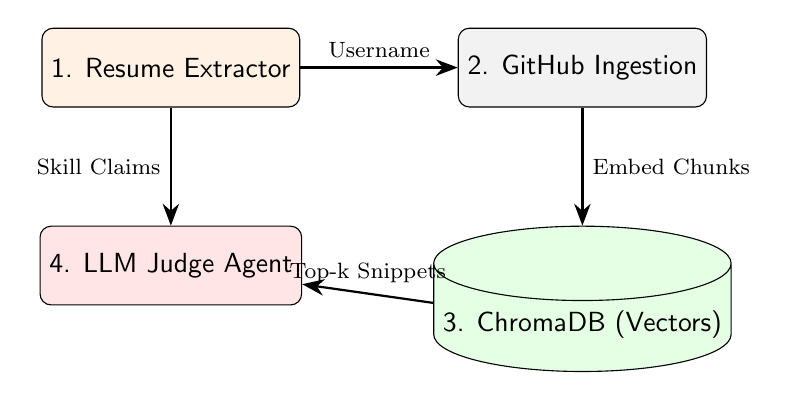
\begin{tikzpicture}[
    node distance=1.5cm and 2cm,
    box/.style={rectangle, draw, rounded corners, fill=blue!10, minimum width=3cm, minimum height=1cm, text centered, font=\sffamily},
    db/.style={cylinder, draw, shape border rotate=90, aspect=0.25, fill=green!10, minimum width=2.5cm, minimum height=1.5cm, text centered, font=\sffamily},
    arrow/.style={-{Stealth[scale=1.2]}, thick}
]

% Nodes
\node (pdf) [box, fill=orange!10] {1. Resume Extractor};
\node (github) [box, fill=gray!10, right=of pdf] {2. GitHub Ingestion};
\node (chroma) [db, below=of github] {3. ChromaDB (Vectors)};
\node (judge) [box, fill=red!10, below=of pdf] {4. LLM Judge Agent};

% Arrows
\draw [arrow] (pdf) -- node[above, font=\footnotesize] {Username} (github);
\draw [arrow] (github) -- node[right, font=\footnotesize] {Embed Chunks} (chroma);
\draw [arrow] (pdf) -- node[left, font=\footnotesize] {Skill Claims} (judge);
\draw [arrow] (chroma) -- node[above, font=\footnotesize] {Top-k Snippets} (judge);

\end{tikzpicture}
\caption{CodeAudit AI System Architecture}
\end{figure}

% ---------------------------------------------------------
\section{5. Prompt Engineering: Chain-of-Thought}
% ---------------------------------------------------------
\subsection{What is Chain-of-Thought (CoT)?}
Normally, if you ask an AI a question, it blurts out the answer immediately. \textbf{Chain-of-Thought} forces the AI to "think out loud" step-by-step before giving the final answer. 
\newline\newline
\textbf{Our CoT Rubric:} The LLM Judge must explicitly look for:
1. Import statements (e.g., \texttt{import tensorflow}).
2. Active framework usage (e.g., \texttt{model.compile()}).
If the skill is only mentioned in a text comment, the Judge must mark it \textit{Unsubstantiated}.

\section{Summary: How to Answer the Toughest Questions}
\begin{itemize}
    \item \textbf{"Did you just wrap an API?"} \newline No. We built a custom Retrieval-Augmented Generation pipeline. The LLM is only the final "judge." The core engineering lies in the asynchronous code ingestion, chunking overlap logic (800 chars with 100 stride), and the dense vector database architecture.
    \item \textbf{"Why not fine-tune a model?"} \newline Fine-tuning teaches a model new style/grammar, but it doesn't teach it new facts efficiently. Candidates update their GitHub daily. RAG allows us to search real-time factual data without retraining a neural network.
    \item \textbf{"How do you handle False Positives?"} \newline By utilizing a zero-temperature (deterministic) LLM combined with strict Chain-of-Thought rubrics, ensuring it only verifies skills if explicit Abstract Syntax Tree (AST) patterns (like function calls) are found in the retrieved chunks.
\end{itemize}

\end{document}
